\chapter{Funciones elementales}
\setcounter{exercicio}{0}



\Exercicio Indica cuál de las siguientes gráficas no corresponde con una función:
	
\begin{enumerate}[topsep=0pt]
	\item \textbf{[C]} 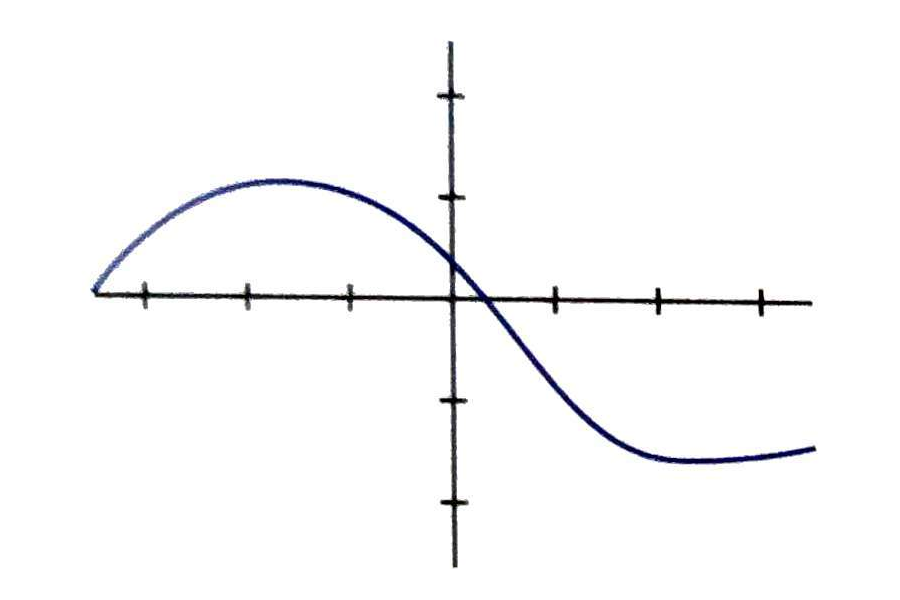
\includegraphics[height=4cm]{../img/funciones-grafica1.png}
	\item \textbf{[C]} 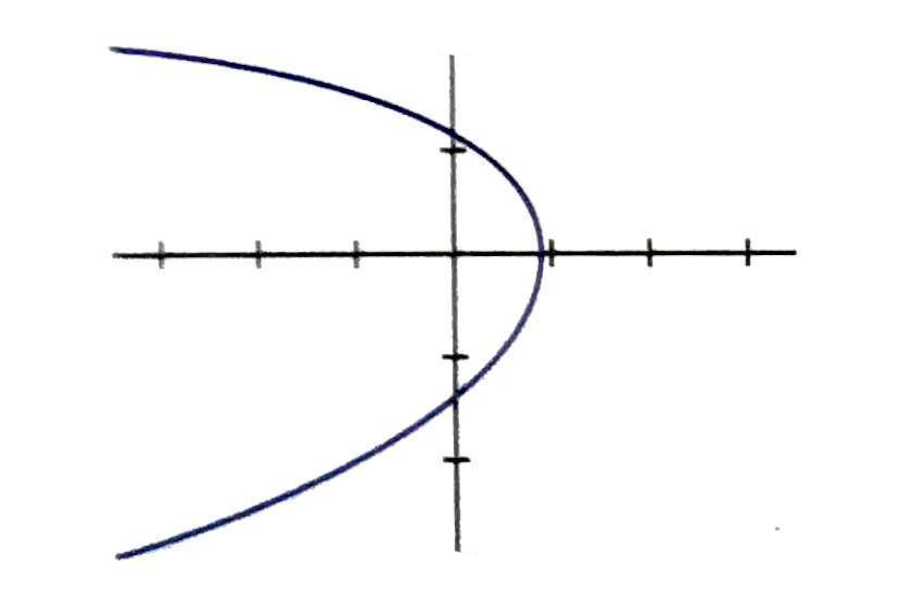
\includegraphics[height=4cm]{../img/funciones-grafica3.png}
	\item 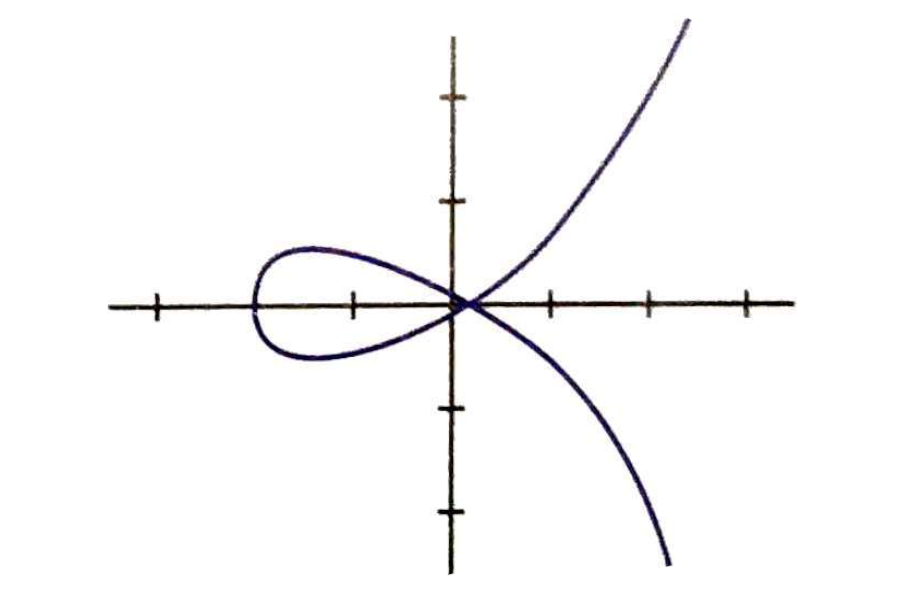
\includegraphics[height=4cm]{../img/funciones-grafica4.png}
	\item 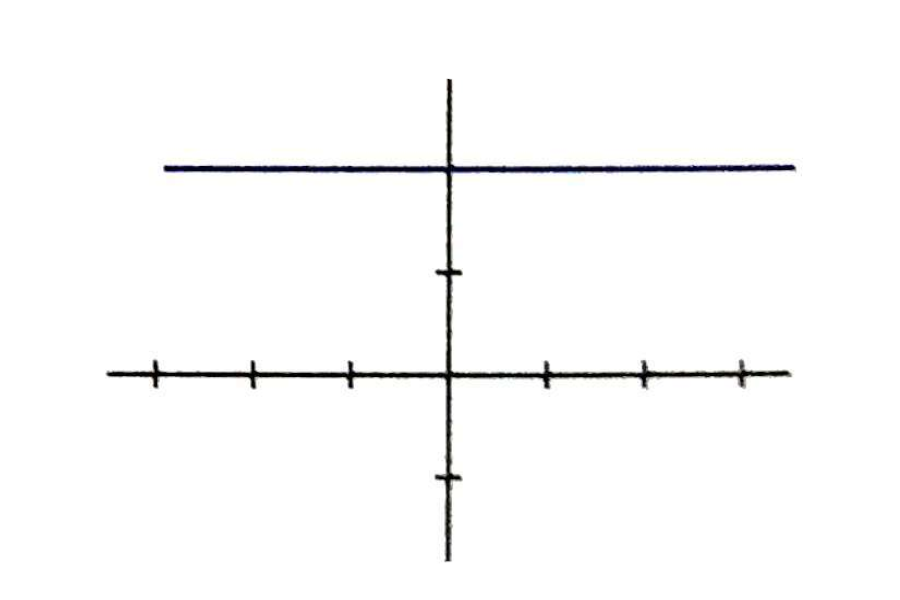
\includegraphics[height=4cm]{../img/funciones-grafica6.png}
\end{enumerate}

\Exercicio Indica el valor de f(3) para cada caso:

\begin{enumerate}[topsep=0pt]
	\item \textbf{[C]} $ f(x) = 3x + 2 $
	\item \textbf{[C]} $ f(x) = x^2 $
	\item \textbf{[C]} $ f(x) = \sqrt{x + 1} $
	\item $f(x) = log(x+7)$
	\item $f(x) = sin(30x)$
	\item $f(x) = 2^x$
\end{enumerate}


\Exercicio Describe las funciones del anexo final de este boletín según los parámetros vistos en clase (\textit{dominio de definición, imagen, puntos de corte con los ejes, continuidad, crecimiento-decrecimiento, máximos y mínimos, simetrías y periodicidad}).

\Exercicio Calcula el dominio y los puntos de corte con los ejes de las siguientes funciones:

\begin{enumerate}[topsep=0pt]
	\item \textbf{[C]} $f(x) = x^2 + 3x$
	\item \textbf{[C]} $g(x) = \sqrt{x^2 - 5x + 4} $
	\item \textbf{[C]} $t(x) = \frac{x^2- 3}{x - 6}$
	\item \textbf{[C]} $s(x) = \frac{\sqrt{2x-3}}{x-10}$
	\item $m(x)= 3x$
	\item $t(x) = \sqrt{x^2 - 4x}$
	\item $g(x) = \frac{x+ 4}{x^2+9}$
	\item $c(x) = \frac{x-4}{\sqrt{x^2-7x+12}}$
	\item $n(x) = \sqrt{\frac{x^2 -4}{x-7}}$
	\item $s(x) = \sqrt{x^3-3x^2-x+3}$
\end{enumerate}


\Exercicio Representa las siguientes funciones polinómicas:

\begin{enumerate}[topsep=0pt]
\item \textbf{[C]} $f(x) = 3x$
	\item \textbf{[C]} $f(x) = -2x + 3$
	\item \textbf{[C]} $f(x) = x^2 - 3x$
	\item \textbf{[C]} $f(x) = 2$
	\item \textbf{[C]} $f(x) = -2x^2 +10x + 12$
	\item \textbf{[C]} $f(x) = x - 4$
	\item  $f(x) = 2x +3$
	\item  $f(x) = x^2 - 2x - 8$
	\item  $f(x) = -3$
	\item  $f(x) = 2x^2 + 6x$
	\item  $f(x) = -3x + 5$
	\item  $f(x) = x^2 -6x + 8$
	\item  $f(x) = 2x - 5$
\end{enumerate}


\Exercicio Indica a que gráfica de las siguientes corresponde las expresiones $f(x) = 2^{x+3}$, $f(x) = ln(x-2)$, $f(x) = x^2+3$,$f(x) = 2x-5$, $f(x) = sin(x) +5$ y $f(x) = -2$   

\begin{enumerate}[topsep=0pt]
	\item \begin{tikzpicture}
		\begin{axis}[
			xmin=-8,xmax=5,
			ymin=-2,ymax=15,
			axis x line=middle,
			axis y line=middle]
			\addplot[
			domain=-8:5,  
			samples=200, 
			color=blue]{2^(x+3)};
		\end{axis}
	\end{tikzpicture}

	\item \begin{tikzpicture}
	\begin{axis}[
		xmin=-6,xmax=6,
		ymin=-1,ymax=7,
		axis x line=middle,
		axis y line=middle]
		\addplot[
		domain=-6:6, 
		samples=200, 
		color=blue]{sin(deg(x)) + 5};
	\end{axis}
	\end{tikzpicture}

	\item \begin{tikzpicture}
	\begin{axis}[
		xmin=-6,xmax=6,
		ymin=-3,ymax=30,
		axis x line=middle,
		axis y line=middle]
		\addplot[
		domain=-6:6, 
		samples=200, 
		color=blue]{x^2 + 3};
	\end{axis}
	\end{tikzpicture}

	\item \begin{tikzpicture}
	\begin{axis}[
		axis x line=middle,
		axis y line=middle]
		\addplot[
		domain=-10:10, 
		samples=200, 
		color=blue]{2*x-5};
	\end{axis}
	\end{tikzpicture}

	\item \begin{tikzpicture}
		\begin{axis}[
			xmin=-1,xmax=6,
			ymin=-7,ymax=5,
			axis x line=middle,
			axis y line=middle]
			\addplot[
			domain=1:6, 
			samples=200, 
			color=blue]{ln(x-2)};
		\end{axis}
	\end{tikzpicture}

	\item \begin{tikzpicture}
		\begin{axis}[
			xmin=-1,xmax=6,
			ymin=-7,ymax=5,
			axis x line=middle,
			axis y line=middle]
			\addplot[
			domain=-2:6, 
			samples=200, 
			color=blue]{-2};
		\end{axis}
	\end{tikzpicture}
\end{enumerate}

\Exercicio Realiza el siguiente Kahoot identificando la expresión que corresponde con cada gráfica según sus propiedades:

\begin{center}
	\qrcode[height=4cm]{https://create.kahoot.it/share/identifica-funciones-elementales/f8e9aee0-d990-4c82-b91f-0cbbd5e556e0}
\end{center}


\Exercicio Representa las siguientes funciones definidas a trozos:

\begin{enumerate}[topsep=0pt]
	\item \textbf{[C]} $f(x) =
		\left\{
			\begin{array}{lcc}
				x - 3 &   si  & x < 5 \\
				4 &  si & x \ge 5
			\end{array}
		\right.$
	\item \textbf{[C]} $t(x) = 
		\left\{
			\begin{array}{lcc}
				x^2 +7x + 10 &   si  & x < -1 \\
				8 &  si & -1 \le x \le 3 \\
				-x + 3 & si & x > 3
			\end{array}
		\right.$
	\item \textbf{[C]} $g(x) = 
		\left\{
			\begin{array}{lcc}
				2x &   si  & x < -4 \\
				4 &  si & -4 \le x < 6 \\
				-x^2 +12x -30 & si & x \ge 6
			\end{array}
		  \right.$
		  
		  
	\item $f(x) = 
		\left\{
		\begin{array}{lcc}
			3x &   si  & x < 4 \\
			x^2 - 3x &    si &  x \ge 4  
		\end{array}
		\right.$		  
	
	\item $f(x) = 
		\left\{
		\begin{array}{lcc}
			3x -2  &   si    & x < 2 \\
			-4x &    si &  x \ge 2  
		\end{array}
		\right.$
		  
	\item $f(x) = 
		\left\{
		\begin{array}{lcc}
			1             &   si  & x < 0 \\
			3x + 2        &   si  & 0 \le x \le 5 \\
			x^2 - 8x + 15 &   si  & x \ge 5
		\end{array}
		\right.$
			  
	\item $f(x) = 
		\left\{
		\begin{array}{lcc}
			x^2 - 3  &  si  & x \le -1 \\
			2        &  si  & -1 < x \le 4 \\
			-x^2 + 2 &  si  & x > 4
		\end{array}
		\right.$
	
	\item $f(x) = 2x - 3 + |2x-3|$
	\item $f(x) = |x+2| + |x+3|$
	\item $f(x) = x +|x-3| + |x+5|$

\end{enumerate}


\Exercicio Dadas las funciones $f(x) = 2x + 3$ , $g(x) = \sqrt{x}$ y $s(x) = x^2$ calcula:

\begin{enumerate}[topsep=0pt]
\item \textbf{[C]} $ (f+g)(x) $
	\item \textbf{[C]} $ (f \cdot g)(x) $
	\item \textbf{[C]} $ (\frac{s}{f})(x)$
	\item \textbf{[C]} $ (g \circ f)(x)$
	\item \textbf{[C]} $ (f \circ s)(x)$
	
	\item  $ (f + s)(x)$
	\item  $ (f \cdot s)(x)$
	\item  $ (\frac{s}{g})(x)$
	\item  $ (f \circ g)(x)$
	\item  $ (g \circ s)(x)$
\end{enumerate}


\Exercicio Calcula la inversa de las siguientes funciones. Comprueba que $(f \circ f^{-1})(x) = (f^{-1} \circ f)(x) = x$:

\begin{enumerate}[topsep=0pt]
	\item \textbf{[C]} $f(x) = (x-2)^2$
	\item \textbf{[C]} $g(x) = \sqrt{x-3} $
	\item \textbf{[C]} $t(x) = \frac{x-1}{x+2}$
	
	\item $f(x) = 1-x^2$
	\item $f(x) = \frac{1}{x^2-4}$
	\item $f(x) = \sqrt{2x-5}$
	\item $f(x) = log(x + 3)$
	\item $f(x) = 2x - 5$
\end{enumerate}